\subsection{Results for Trajectories Estimated Using $x$ and $y$ Offset}
%\label{subsec:no_abs_results}
%\vspace{10pt}

Figure~\ref{fig:best_R2_traj_val} contains the average $R^{2}$ (\%) across $k$-fold testing datasets using different trajectory estimation methods, validation datasets for all trajectories estimated in nested $k$-fold cross-validation by different trajectory estimation methods, RNN models, and forecasting times.

\begin{figure}[!ht]
	\centering
	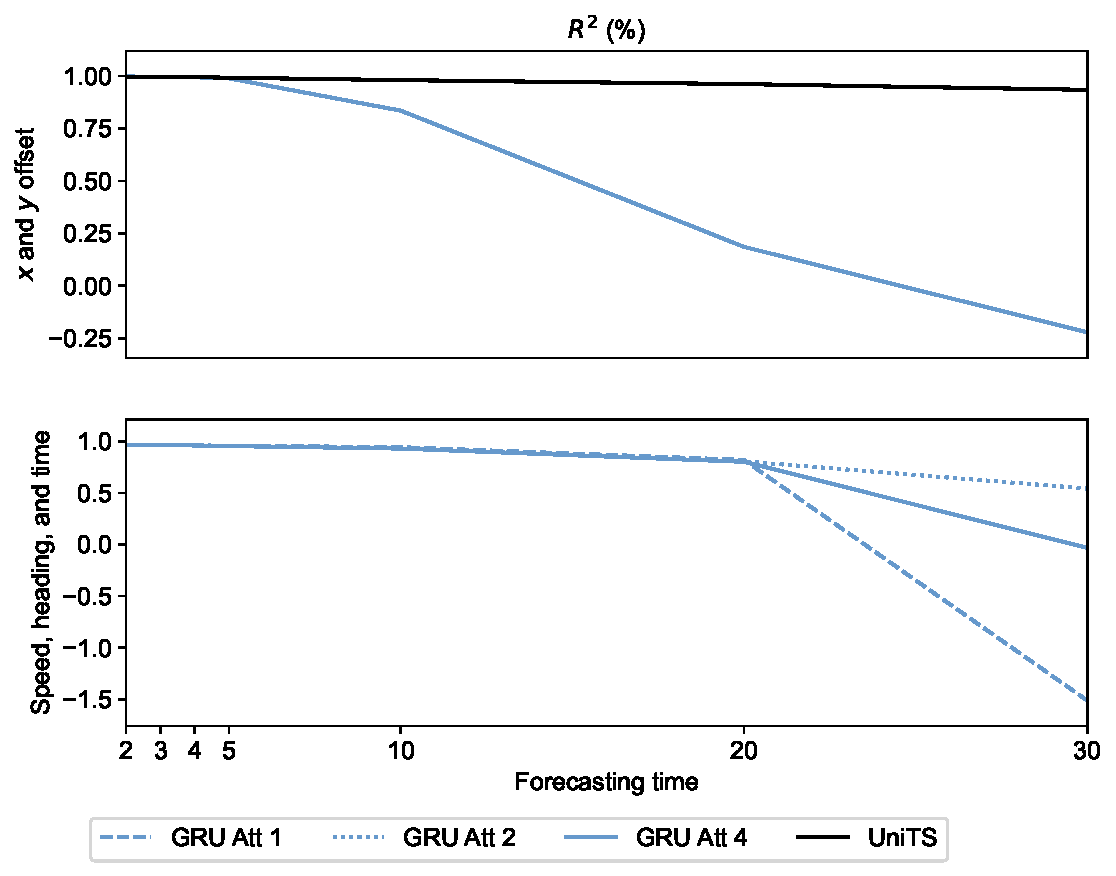
\includegraphics[width = 0.99 \linewidth]{best_R2_traj_val.pdf}
	\caption{The average $R^{2}$ (\%) across $k$-fold testing datasets using different trajectory estimation methods, validation datasets for all trajectories estimated in nested $k$-fold cross-validation by different trajectory estimation methods, RNN models, and forecasting times.}
	\label{fig:best_R2_traj_val}
\end{figure}

The average $R^{2}$ (\%), with standard deviation in brackets, across $k$-fold validation datasets for the trajectories in the $k$-fold testing datasets estimated using $x$ and $y$ offset, different RNN models, and forecasting times is listed in Table~\ref{tab:best_no_abs_R2}.

\begin{table}[!ht]
	\centering
	\resizebox{\linewidth}{!}{
		\begin{tabular}{|c|c|c|c|c|c|c|c|}
			\hline
			Model & $2$ $s$ & $3$ $s$ & $4$ $s$ & $5$ $s$ & $10$ $s$ & $20$ $s$ & $30$ $s$ \\ \hline
			\multirow{2}{*}{GRU Att 4} & $\mathbf{99.75\%}$ & $\mathbf{99.59\%}$ & $99.38\%$ & $98.86\%$ & $83.46\%$ & $18.51\%$ & $-22.18\%$ \\
			 & \textbf{(}$\mathbf{0.11\%}$\textbf{)} & \textbf{(}$\mathbf{0.14\%}$\textbf{)} & ($0.23\%$) & ($0.61\%$) & ($11.42\%$) & ($33.32\%$) & ($76.47\%$) \\ \hline
			\multirow{2}{*}{UniTS} & $99.31\%$ & $99.33\%$ & $\mathbf{99.45\%}$ & $\mathbf{99.15\%}$ & $\mathbf{98.01\%}$ & $\mathbf{96.12\%}$ & $\mathbf{93.37\%}$ \\
			 & ($1.54\%$) & ($1.13\%$) & \textbf{(}$\mathbf{0.2\%}$\textbf{)} & \textbf{(}$\mathbf{0.4\%}$\textbf{)} & \textbf{(}$\mathbf{0.77\%}$\textbf{)} & \textbf{(}$\mathbf{1.27\%}$\textbf{)} & \textbf{(}$\mathbf{2.52\%}$\textbf{)} \\ \hline
		\end{tabular}
	}
	\caption{The average $R^{2}$ (\%), with standard deviation in brackets, across $k$-fold validation datasets for the trajectories in the $k$-fold testing datasets estimated using $x$ and $y$ offset, different RNN models, and forecasting times.}
	\label{tab:best_no_abs_R2}
\end{table}

The GRU Att 4 model achieved the highest $R^{2}$ (\%) for trajectories estimated using $x$ and $y$ offset, and a forecasting time of $2$, and $3$ $s$ with average values and standard deviation (in brackets) that equal $99.75$\% ($0.11$\%), and $99.59$\% ($0.14$\%) respectively.

The UniTS model achieved the highest $R^{2}$ (\%) for trajectories estimated using $x$ and $y$ offset, and a forecasting time of $4$, $5$, $10$, $20$, and $30$ $s$ with average values and standard deviation (in brackets) that equal $99.45$\% ($0.2$\%), $99.15$\% ($0.4$\%), $98.01$\% ($0.77$\%), $96.12$\% ($1.27$\%), and $93.37$\% ($2.52$\%) respectively.

Figure~\ref{fig:best_MAE_traj_val} contains the average MAE across $k$-fold testing datasets using different trajectory estimation methods, validation datasets for all trajectories estimated in nested $k$-fold cross-validation by different trajectory estimation methods, RNN models, and forecasting times.

\begin{figure}[!ht]
	\centering
	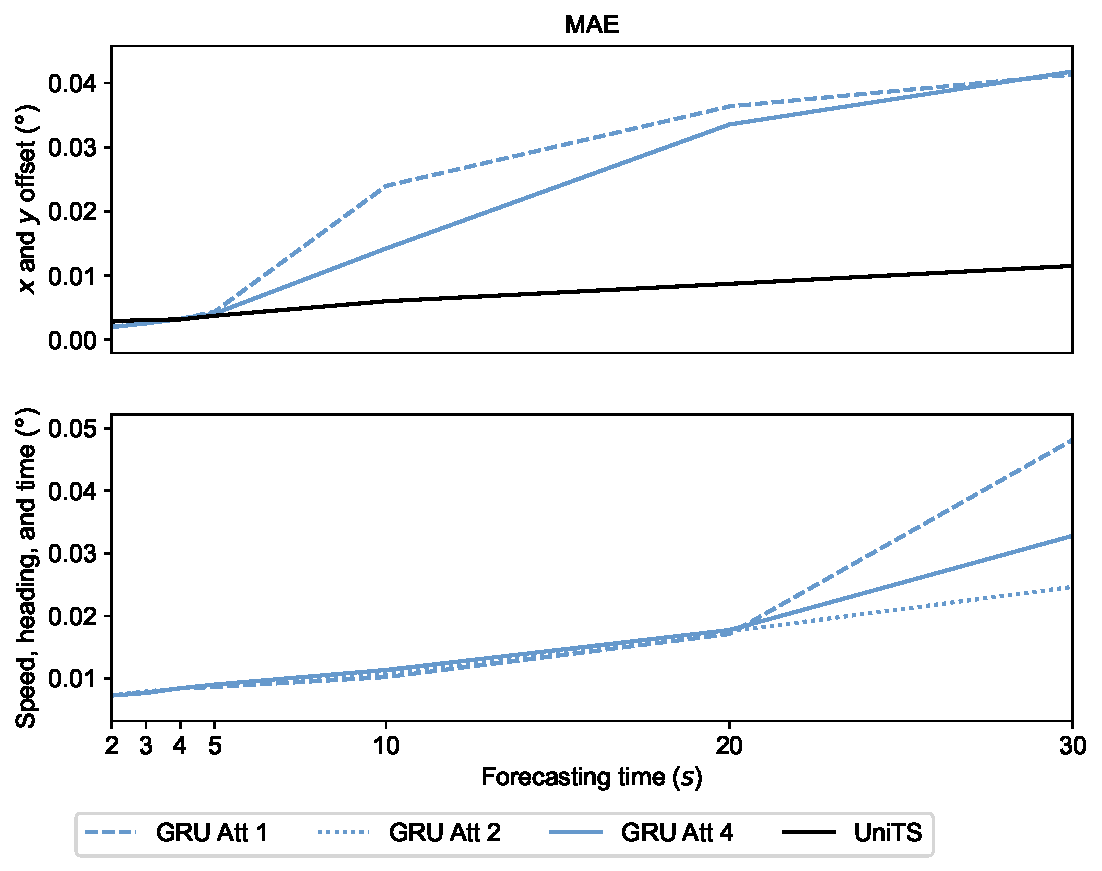
\includegraphics[width = 0.99 \linewidth]{best_MAE_traj_val.pdf}
	\caption{The average MAE across $k$-fold testing datasets using different trajectory estimation methods, validation datasets for all trajectories estimated in nested $k$-fold cross-validation by different trajectory estimation methods, RNN models, and forecasting times.}
	\label{fig:best_MAE_traj_val}
\end{figure}

The average MAE in $\degree$ ($\times 10^{-3}$), with standard deviation in brackets, across $k$-fold validation datasets for the trajectories in the $k$-fold testing datasets estimated using $x$ and $y$ offset, different RNN models, and forecasting times is listed in Table~\ref{tab:best_no_abs_MAE}.

\begin{table}[!ht]
	\centering
	\resizebox{\linewidth}{!}{
		\begin{tabular}{|c|c|c|c|c|c|c|c|}
			\hline
			Model & $2$ $s$ & $3$ $s$ & $4$ $s$ & $5$ $s$ & $10$ $s$ & $20$ $s$ & $30$ $s$ \\ \hline
			\multirow{2}{*}{GRU Att 1} & $2.07$ & $\mathbf{2.54}$ & $3.25$ & $4.36$ & $23.98$ & $36.35$ & $41.33$ \\
			 & ($0.23$) & \textbf{(}$\mathbf{0.28}$\textbf{)} & ($0.4$) & ($0.84$) & ($5.44$) & ($9.41$) & ($7.37$) \\ \hline
			\multirow{2}{*}{GRU Att 4} & $\mathbf{1.95}$ & $2.56$ & $3.22$ & $4.08$ & $14.23$ & $33.54$ & $41.8$ \\
			 & \textbf{(}$\mathbf{0.27}$\textbf{)} & ($0.29$) & ($0.31$) & ($0.41$) & ($3.09$) & ($4.46$) & ($9.25$) \\ \hline
			\multirow{2}{*}{UniTS} & $2.83$ & $3.12$ & $\mathbf{3.17}$ & $\mathbf{3.75}$ & $\mathbf{6.0}$ & $\mathbf{8.71}$ & $\mathbf{11.51}$ \\
			 & ($2.33$) & ($2.14$) & \textbf{(}$\mathbf{0.39}$\textbf{)} & \textbf{(}$\mathbf{0.58}$\textbf{)} & \textbf{(}$\mathbf{0.65}$\textbf{)} & \textbf{(}$\mathbf{0.8}$\textbf{)} & \textbf{(}$\mathbf{1.04}$\textbf{)} \\ \hline
		\end{tabular}
	}
	\caption{The average MAE in $\degree$ ($\times 10^{-3}$), with standard deviation in brackets, across $k$-fold validation datasets for the trajectories in the $k$-fold testing datasets estimated using $x$ and $y$ offset, different RNN models, and forecasting times.}
	\label{tab:best_no_abs_MAE}
\end{table}

The GRU Att 1 model achieved the lowest MAE for trajectories estimated using $x$ and $y$ offset, and a forecasting time of $3$ $s$ with an average value and standard deviation (in brackets) that equals $2.54 \times 10^{-3}$ $\degree$ ($0.28 \times 10^{-3}$ $\degree$).

The GRU Att 4 model achieved the lowest MAE for trajectories estimated using $x$ and $y$ offset, and a forecasting time of $2$ $s$ with an average value and standard deviation (in brackets) that equals $1.95 \times 10^{-3}$ $\degree$ ($0.27 \times 10^{-3}$ $\degree$).

The UniTS model achieved the lowest MAE for trajectories estimated using $x$ and $y$ offset, and a forecasting time of $4$, $5$, $10$, $20$, and $30$ $s$ with average values and standard deviation (in brackets) that equal $3.17 \times 10^{-3}$ $\degree$ ($0.39 \times 10^{-3}$ $\degree$), $3.75 \times 10^{-3}$ $\degree$ ($0.58 \times 10^{-3}$ $\degree$), $6.0 \times 10^{-3}$ $\degree$ ($0.65 \times 10^{-3}$ $\degree$), $8.71 \times 10^{-3}$ $\degree$ ($0.8 \times 10^{-3}$ $\degree$), and $11.51 \times 10^{-3}$ $\degree$ ($1.04 \times 10^{-3}$ $\degree$) respectively.

Figure~\ref{fig:best_haversine_traj_val} contains the average haversine distance in $km$ across $k$-fold testing datasets using different trajectory estimation methods, validation datasets for all trajectories estimated in nested $k$-fold cross-validation by different trajectory estimation methods, RNN models, and forecasting times.

\begin{figure}[!ht]
	\centering
	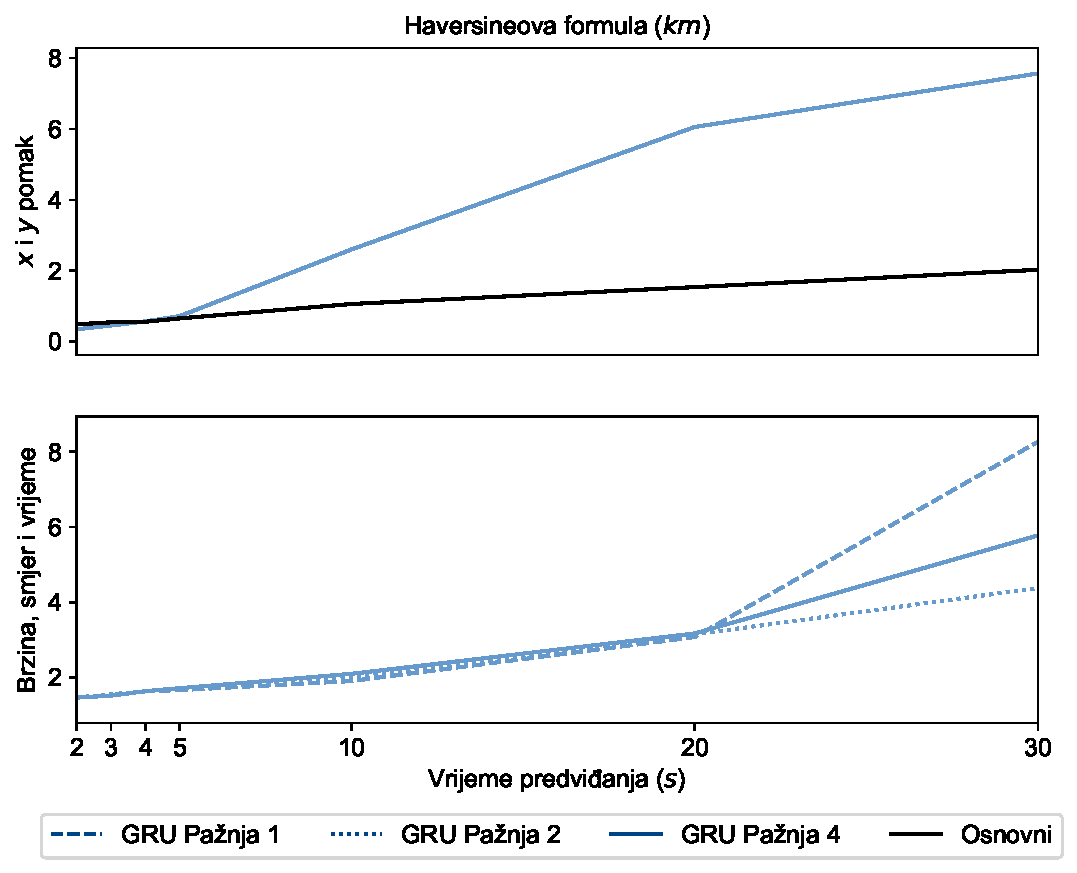
\includegraphics[width = 0.99 \linewidth]{best_haversine_traj_val.pdf}
	\caption{The average haversine distance in $km$ across $k$-fold testing datasets using different trajectory estimation methods, validation datasets for all trajectories estimated in nested $k$-fold cross-validation by different trajectory estimation methods, RNN models, and forecasting times.}
	\label{fig:best_haversine_traj_val}
\end{figure}

The average haversine distance in $km$, with standard deviation in brackets, across $k$-fold validation datasets for the trajectories in the $k$-fold testing datasets estimated using $x$ and $y$ offset, different RNN models, and forecasting times is listed in Table~\ref{tab:best_no_abs_haversine}.

\begin{table}[!ht]
	\centering
	\resizebox{\linewidth}{!}{
		\begin{tabular}{|c|c|c|c|c|c|c|c|}
			\hline
			Model & $2$ $s$ & $3$ $s$ & $4$ $s$ & $5$ $s$ & $10$ $s$ & $20$ $s$ & $30$ $s$ \\ \hline
			\multirow{2}{*}{GRU Att 4} & $\mathbf{0.346}$ & $\mathbf{0.452}$ & $0.569$ & $0.719$ & $2.599$ & $6.056$ & $7.567$ \\
			 & \textbf{(}$\mathbf{0.046}$\textbf{)} & \textbf{(}$\mathbf{0.052}$\textbf{)} & ($0.055$) & ($0.073$) & ($0.577$) & ($0.834$) & ($1.868$) \\ \hline
			\multirow{2}{*}{UniTS} & $0.485$ & $0.542$ & $\mathbf{0.558}$ & $\mathbf{0.653}$ & $\mathbf{1.059}$ & $\mathbf{1.536}$ & $\mathbf{2.025}$ \\
			 & ($0.365$) & ($0.338$) & \textbf{(}$\mathbf{0.071}$\textbf{)} & \textbf{(}$\mathbf{0.098}$\textbf{)} & \textbf{(}$\mathbf{0.124}$\textbf{)} & \textbf{(}$\mathbf{0.157}$\textbf{)} & \textbf{(}$\mathbf{0.209}$\textbf{)} \\ \hline
		\end{tabular}
	}
	\caption{The average haversine distance in $km$, with standard deviation in brackets, across $k$-fold validation datasets for the trajectories in the $k$-fold testing datasets estimated using $x$ and $y$ offset, different RNN models, and forecasting times.}
	\label{tab:best_no_abs_haversine}
\end{table}

The GRU Att 4 model achieved the lowest haversine distance for trajectories estimated using $x$ and $y$ offset, and a forecasting time of $2$, and $3$ $s$ with average values and standard deviation (in brackets) that equal $0.346$ $km$ ($0.046$ $km$), and $0.452$ $km$ ($0.052$ $km$) respectively.

The UniTS model achieved the lowest haversine distance for trajectories estimated using $x$ and $y$ offset, and a forecasting time of $4$, $5$, $10$, $20$, and $30$ $s$ with average values and standard deviation (in brackets) that equal $0.558$ $km$ ($0.071$ $km$), $0.653$ $km$ ($0.098$ $km$), $1.059$ $km$ ($0.124$ $km$), $1.536$ $km$ ($0.157$ $km$), and $2.025$ $km$ ($0.209$ $km$) respectively.

\subsection{Results for Trajectories Estimated Using Speed, Heading, and Time}
%\label{subsec:speed_actual_dir_results}
%\vspace{10pt}

The average $R^{2}$ (\%), with standard deviation in brackets, across $k$-fold validation datasets for the trajectories in the $k$-fold testing datasets estimated using speed, heading, and time, different RNN models, and forecasting times is listed in Table~\ref{tab:best_speed_actual_dir_R2}.

\begin{table}[!ht]
	\centering
	\resizebox{\linewidth}{!}{
		\begin{tabular}{|c|c|c|c|c|c|c|c|}
			\hline
			Model & $2$ $s$ & $3$ $s$ & $4$ $s$ & $5$ $s$ & $10$ $s$ & $20$ $s$ & $30$ $s$ \\ \hline
			\multirow{2}{*}{GRU Att 1} & $96.53\%$ & $96.303\%$ & $95.928\%$ & $\mathbf{95.699\%}$ & $\mathbf{94.222\%}$ & $\mathbf{81.816\%}$ & $-151.278\%$ \\
			 & ($0.211\%$) & ($0.233\%$) & ($0.336\%$) & \textbf{(}$\mathbf{0.445\%}$\textbf{)} & \textbf{(}$\mathbf{1.083\%}$\textbf{)} & \textbf{(}$\mathbf{6.541\%}$\textbf{)} & ($454.465\%$) \\ \hline
			\multirow{2}{*}{GRU Att 2} & $96.526\%$ & $96.205\%$ & $95.862\%$ & $95.398\%$ & $93.415\%$ & $80.484\%$ & $\mathbf{54.101\%}$ \\
			 & ($0.161\%$) & ($0.303\%$) & ($0.482\%$) & ($0.959\%$) & ($2.341\%$) & ($8.479\%$) & \textbf{(}$\mathbf{25.777\%}$\textbf{)} \\ \hline
			\multirow{2}{*}{GRU Att 4} & $\mathbf{96.554\%}$ & $\mathbf{96.359\%}$ & $\mathbf{95.93\%}$ & $95.334\%$ & $92.902\%$ & $80.1\%$ & $-3.241\%$ \\
			 & \textbf{(}$\mathbf{0.204\%}$\textbf{)} & \textbf{(}$\mathbf{0.243\%}$\textbf{)} & \textbf{(}$\mathbf{0.4\%}$\textbf{)} & ($0.53\%$) & ($1.989\%$) & ($7.486\%$) & ($190.754\%$) \\ \hline
		\end{tabular}
	}
	\caption{The average $R^{2}$ (\%), with standard deviation in brackets, across $k$-fold validation datasets for the trajectories in the $k$-fold testing datasets estimated using speed, heading, and time, different RNN models, and forecasting times.}
	\label{tab:best_speed_actual_dir_R2}
\end{table}

The GRU Att 1 model achieved the highest $R^{2}$ (\%) for trajectories estimated using speed, heading, and time, and a forecasting time of $10$, $20$, and $5$ $s$ with average values and standard deviation (in brackets) that equal $94.22$\% ($1.08$\%), $81.82$\% ($6.54$\%), and $95.7$\% ($0.44$\%) respectively.

The GRU Att 2 model achieved the highest $R^{2}$ (\%) for trajectories estimated using speed, heading, and time, and a forecasting time of $30$ $s$ with an average value and standard deviation (in brackets) that equals $54.1$\% ($25.78$\%).

The GRU Att 4 model achieved the highest $R^{2}$ (\%) for trajectories estimated using speed, heading, and time, and a forecasting time of $2$, $3$, and $4$ $s$ with average values and standard deviation (in brackets) that equal $96.55$\% ($0.2$\%), $96.36$\% ($0.24$\%), and $95.93$\% ($0.4$\%) respectively.

The average MAE in $\degree$ ($\times 10^{-3}$), with standard deviation in brackets, across $k$-fold validation datasets for the trajectories in the $k$-fold testing datasets estimated using speed, heading, and time, different RNN models, and forecasting times is listed in Table~\ref{tab:best_speed_actual_dir_MAE}.

\begin{table}[!ht]
	\centering
	\resizebox{\linewidth}{!}{
		\begin{tabular}{|c|c|c|c|c|c|c|c|}
			\hline
			Model & $2$ $s$ & $3$ $s$ & $4$ $s$ & $5$ $s$ & $10$ $s$ & $20$ $s$ & $30$ $s$ \\ \hline
			\multirow{2}{*}{GRU Att 1} & $7.298$ & $7.77$ & $\mathbf{8.419}$ & $\mathbf{8.638}$ & $\mathbf{10.223}$ & $\mathbf{17.111}$ & $48.15$ \\
			 & ($0.407$) & ($0.337$) & \textbf{(}$\mathbf{0.385}$\textbf{)} & \textbf{(}$\mathbf{0.449}$\textbf{)} & \textbf{(}$\mathbf{0.618}$\textbf{)} & \textbf{(}$\mathbf{1.225}$\textbf{)} & ($38.906$) \\ \hline
			\multirow{2}{*}{GRU Att 2} & $7.308$ & $7.924$ & $8.442$ & $8.803$ & $10.78$ & $17.518$ & $\mathbf{24.644}$ \\
			 & ($0.373$) & ($0.53$) & ($0.491$) & ($0.584$) & ($1.085$) & ($1.404$) & \textbf{(}$\mathbf{3.038}$\textbf{)} \\ \hline
			\multirow{2}{*}{GRU Att 4} & $\mathbf{7.267}$ & $\mathbf{7.674}$ & $8.444$ & $9.031$ & $11.367$ & $17.745$ & $32.805$ \\
			 & \textbf{(}$\mathbf{0.369}$\textbf{)} & \textbf{(}$\mathbf{0.397}$\textbf{)} & ($0.414$) & ($0.438$) & ($0.984$) & ($1.489$) & ($26.7$) \\ \hline
		\end{tabular}
	}
	\caption{The average MAE in $\degree$ ($\times 10^{-3}$), with standard deviation in brackets, across $k$-fold validation datasets for the trajectories in the $k$-fold testing datasets estimated using speed, heading, and time, different RNN models, and forecasting times.}
	\label{tab:best_speed_actual_dir_MAE}
\end{table}

The GRU Att 1 model achieved the lowest MAE for trajectories estimated using speed, heading, and time, and a forecasting time of $10$, $20$, $4$, and $5$ $s$ with average values and standard deviation (in brackets) that equal $10.22 \times 10^{-3}$ $\degree$ ($0.62 \times 10^{-3}$ $\degree$), $17.11 \times 10^{-3}$ $\degree$ ($1.22 \times 10^{-3}$ $\degree$), $8.42 \times 10^{-3}$ $\degree$ ($0.39 \times 10^{-3}$ $\degree$), and $8.64 \times 10^{-3}$ $\degree$ ($0.45 \times 10^{-3}$ $\degree$) respectively.

The GRU Att 2 model achieved the lowest MAE for trajectories estimated using speed, heading, and time, and a forecasting time of $30$ $s$ with an average value and standard deviation (in brackets) that equals $24.64 \times 10^{-3}$ $\degree$ ($3.04 \times 10^{-3}$ $\degree$).

The GRU Att 4 model achieved the lowest MAE for trajectories estimated using speed, heading, and time, and a forecasting time of $2$, and $3$ $s$ with average values and standard deviation (in brackets) that equal $7.27 \times 10^{-3}$ $\degree$ ($0.37 \times 10^{-3}$ $\degree$), and $7.67 \times 10^{-3}$ $\degree$ ($0.4 \times 10^{-3}$ $\degree$) respectively.

The average haversine distance in $km$, with standard deviation in brackets, across $k$-fold validation datasets for the trajectories in the $k$-fold testing datasets estimated using speed, heading, and time, different RNN models, and forecasting times is listed in Table~\ref{tab:best_speed_actual_dir_haversine}.

\begin{table}[!ht]
	\centering
	\resizebox{\linewidth}{!}{
		\begin{tabular}{|c|c|c|c|c|c|c|c|}
			\hline
			Model & $2$ $s$ & $3$ $s$ & $4$ $s$ & $5$ $s$ & $10$ $s$ & $20$ $s$ & $30$ $s$ \\ \hline
			\multirow{2}{*}{GRU Att 1} & $1.474$ & $1.532$ & $1.637$ & $\mathbf{1.665}$ & $\mathbf{1.906}$ & $\mathbf{3.075}$ & $8.261$ \\
			 & ($0.09$) & ($0.081$) & ($0.082$) & \textbf{(}$\mathbf{0.083}$\textbf{)} & \textbf{(}$\mathbf{0.116}$\textbf{)} & \textbf{(}$\mathbf{0.202}$\textbf{)} & ($6.403$) \\ \hline
			\multirow{2}{*}{GRU Att 2} & $1.47$ & $1.554$ & $\mathbf{1.634}$ & $1.681$ & $2.001$ & $3.145$ & $\mathbf{4.38}$ \\
			 & ($0.086$) & ($0.109$) & \textbf{(}$\mathbf{0.095}$\textbf{)} & ($0.108$) & ($0.191$) & ($0.232$) & \textbf{(}$\mathbf{0.515}$\textbf{)} \\ \hline
			\multirow{2}{*}{GRU Att 4} & $\mathbf{1.467}$ & $\mathbf{1.518}$ & $1.638$ & $1.716$ & $2.098$ & $3.17$ & $5.773$ \\
			 & \textbf{(}$\mathbf{0.084}$\textbf{)} & \textbf{(}$\mathbf{0.092}$\textbf{)} & ($0.089$) & ($0.086$) & ($0.169$) & ($0.248$) & ($4.507$) \\ \hline
		\end{tabular}
	}
	\caption{The average haversine distance in $km$, with standard deviation in brackets, across $k$-fold validation datasets for the trajectories in the $k$-fold testing datasets estimated using speed, heading, and time, different RNN models, and forecasting times.}
	\label{tab:best_speed_actual_dir_haversine}
\end{table}

The GRU Att 1 model achieved the lowest haversine distance for trajectories estimated using speed, heading, and time, and a forecasting time of $10$, $20$, and $5$ $s$ with average values and standard deviation (in brackets) that equal $1.906$ $km$ ($0.116$ $km$), $3.075$ $km$ ($0.202$ $km$), and $1.665$ $km$ ($0.083$ $km$) respectively.

The GRU Att 2 model achieved the lowest haversine distance for trajectories estimated using speed, heading, and time, and a forecasting time of $30$, and $4$ $s$ with average values and standard deviation (in brackets) that equal $4.38$ $km$ ($0.515$ $km$), and $1.634$ $km$ ($0.095$ $km$) respectively.

The GRU Att 4 model achieved the lowest haversine distance for trajectories estimated using speed, heading, and time, and a forecasting time of $2$, and $3$ $s$ with average values and standard deviation (in brackets) that equal $1.467$ $km$ ($0.084$ $km$), and $1.518$ $km$ ($0.092$ $km$) respectively.

